%Beamer class
\documentclass{beamer}

\usepackage[czech]{babel}
\usepackage[cp1250]{inputenc}
\usepackage{fontenc}
\usepackage{tgheros}
\usepackage{array}
\usepackage{color}
\usepackage{hyperref}

\usetheme{Antibes}
\usecolortheme{crane}


\title[BE1M13VES]{BE1M13VES}
\subtitle[Manufacturing of Electrical Components] {Manufacturing of Electrical Components}
\author[Brejcha]{Michal Brejcha}
\institute[CTU]{CTU in Prague}
\date[Prague, 2017]{Prague, 2017}

\begin{document}
%------------------------------------------------------------------------------
%Uvodni slajd
%------------------------------------------------------------------------------
\frame{\titlepage}

\begin{frame}
\frametitle{Overview} 
\tableofcontents
\end{frame}

\AtBeginSection[]
{
  \begin{frame}
    \frametitle{TOPIC}
    \tableofcontents[currentsection]
  \end{frame}
}

%------------------------------------------------------------------------------
%Frquency dependency of resistors
%------------------------------------------------------------------------------
\section{\texorpdfstring{Semiconductor Components}{Semiconductor Components}}
%------------------------------------------------------------------------------
	\begin{frame}
    \frametitle{Basic Properties}
		\begin{itemize}
		\item Nonlinear characteristics - used for rectifying, sensing, saturation etc.
		\item VA characteristics are quite dependent on ambient factors - temperature, light.
		\item Some components are able to amplify the input signal - transistors
		\end{itemize}
		
	\end{frame}
%------------------------------------------------------------------------------
	\begin{frame}
    \frametitle{Equivalent Circuit}
		
		For AC circuits the parasitic serial inductance and parallel capacity must be taken into account. The frequency dependence of the resistors is caused especially by its construction.
		\begin{center}
			\begin{tabular}{m{0.45\linewidth} m{0.45\linewidth}}
			%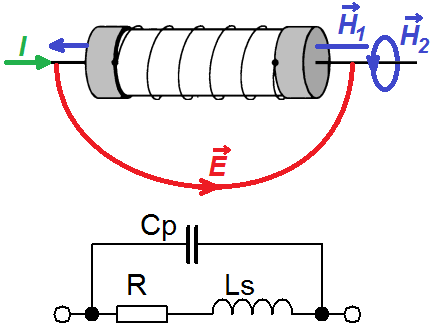
\includegraphics[scale=0.4]{obr01_poleRes.png} &
			
			\begin{itemize}
				\item $H_1$, $H_2$... magnetic field from resistive track and leads.
				\item $E$... electric field (capacitance) between opposite sides of package and leads.
			\end{itemize}
			\end{tabular}
		\end{center}
	\end{frame}
%------------------------------------------------------------------------------
\end{document}